\documentclass{cmc}
\usepackage{amsmath}

\begin{document}


\pagestyle{fancy}
\lhead{\textit{\textbf{Computational Motor Control, Spring 2020} \\
    Python exercise, Lab 6, GRADED}} \rhead{Jon Märki, Jérôme Savary, Gabriel Tornare}

\section*{Student names: Jon Märki, Jérôme Savary, Gabriel Tornare}

\section*{Exercise 2 : Pendulum model with Muscles}


\subsection*{2a. For the given default set of attachment points,
  compute and plot the muscle length and moment arm as a function of
  $\theta$ between $[pi/4, 3pi/4]$ using previous equations and discuss how it influences the pendulum resting position and the torques muscles can apply at different 
  joint angles. You are free to implement this code by yourself as it
  does not have any other dependencies.}
\label{sec:2a}

%===========================================================
%BEGIN USER CODE
%===========================================================

The result of the measures based on the given equations can be observed in figure \ref{fig:2a}. By changing the angle of the arm, we also change the lengths of both muscles, therefore the force they can apply, and finally therefore the torque, which also varies with the moment arm. The resting position == the resting angle is the one at which both muscles, given their respective lengths and stimulations, apply the same opposed torques = no resulting torque.

%TODO : discuss the influence on the resting position and the torque

\begin{figure}[H]
  \centering
  \begin{subfigure}[b]{0.48\textwidth}
    { \centering
      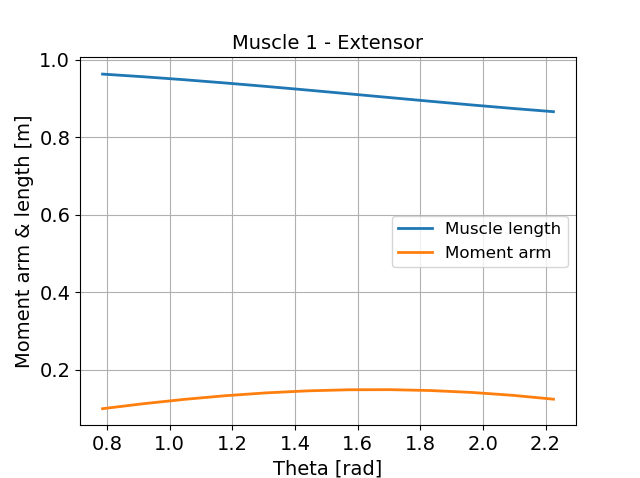
\includegraphics[width=\textwidth]{figures/2a_Length_and_Moment_Arm_m1.png} }
    \caption{Result of experiment 2a on muscle 1.}
    \label{fig:2a_M1}
  \end{subfigure}
  \begin{subfigure}[b]{0.48\textwidth}
    { \centering
      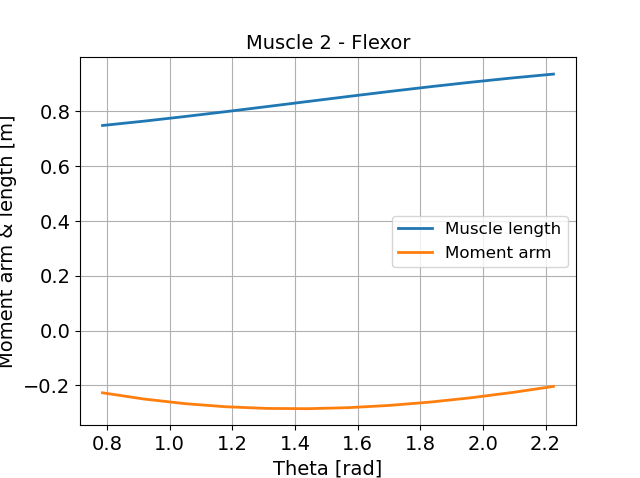
\includegraphics[width=\textwidth]{figures/2a_Length_and_Moment_Arm_m2.png} }
    \caption{Result of experiment on muscle 2.}
    \label{fig:2a_m2}
  \end{subfigure}
  \caption{Result of experiment 2a.}
  \label{fig:2a}
\end{figure}
%===========================================================
%END USER CODE
%===========================================================

\subsection*{2b. Using simple activation wave forms (example : sine or
  square waves) applied to muscles (use
  \fileref{system\_simulation.py::add\_muscle\_stimulations} method in
  \fileref{exercise2.py}), try to obtain a limit cycle behavior for
  the pendulum. Use relevant plots to prove the limit cycle behavior.
  Explain and show the activations wave forms you used. Use
  \fileref{pendulum\_system.py::\-PendulumSystem::\-pendulum\_system}
  function to perturb the model.}
\label{sec:2b}

%===========================================================
%BEGIN USER CODE
%===========================================================

For this part, we inputed the three different signals at two different frequencies (1 and 10 [Hz]). Our 1[Hz] signals can be visualised on Figure \ref{fig:2b_signals}.

\begin{figure}[H]
  \centering
  \begin{subfigure}[b]{0.48\textwidth}
    { \centering
      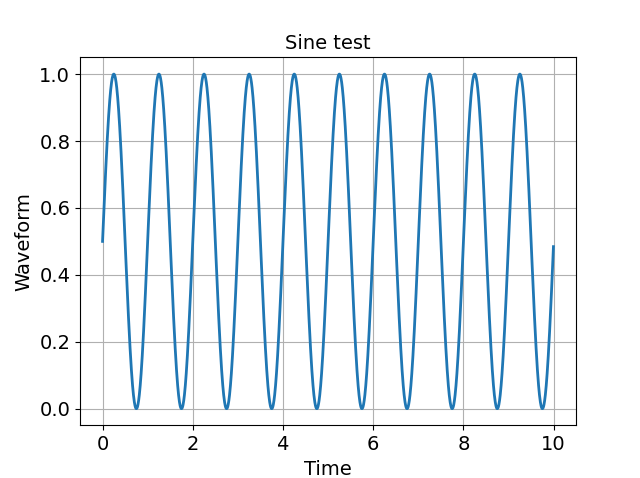
\includegraphics[width=0.99\textwidth]{figures/2b_Sine_test.png} }
    \caption{1[Hz] Sine-shaped stimulation input signal.}
    \label{fig:2b_sine_signal}
  \end{subfigure}
  \begin{subfigure}[b]{0.48\textwidth}
    { \centering
      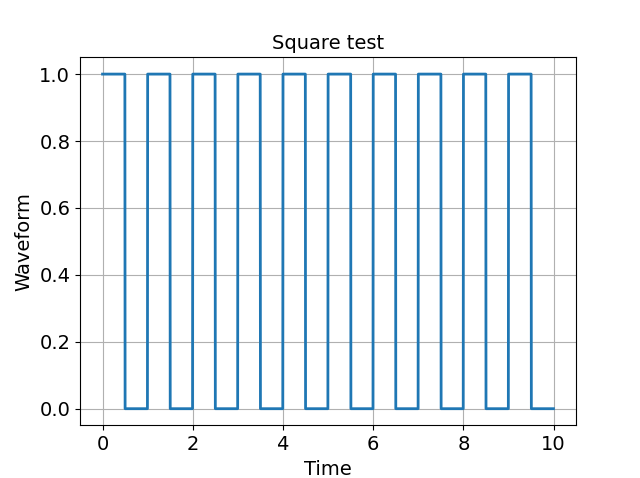
\includegraphics[width=0.99\textwidth]{figures/2b_Square_test.png} }
    \caption{1[Hz] Square-shaped stimulation input signal.}
    \label{fig:2b_sine_phase}
  \end{subfigure}
  
  \begin{subfigure}[b]{0.48\textwidth}
    { \centering
      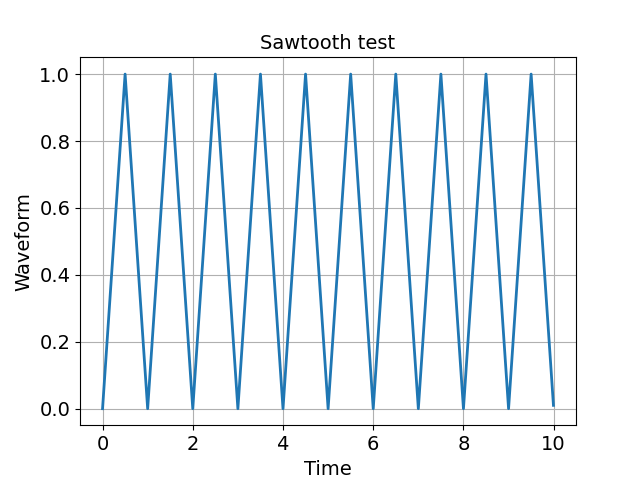
\includegraphics[width=0.99\textwidth]{figures/2b_Sawtooth_test.png} }
    \caption{1[Hz] Sawtooth-shaped stimulation input signal.}
    \label{fig:2b_square_signal}
  \end{subfigure}

  \caption{1[Hz] signals for exercise 2b.}
  \label{fig:2b_signals}
\end{figure}


The result of the measures based on the given equations can be observed in figure \ref{fig:2b} on page \pageref{fig:2b}. We can observe from these measures that the pendulum reaches a limit circle which is about in the same order of magnitude for the three signals, and the measurements from the sineè and sawtooth-shaped signals share more similarities than the ones from the square-shaped one (logically, since they are more similar).
Each stimulation signal has two phase pendulum phases measured: one when the stimulation signals for the flexor and extendor muscles are in phase (left), the other when they are in counterphase (right)

\begin{figure}[H]
  \centering
  \begin{subfigure}[b]{0.48\textwidth}
    { \centering
      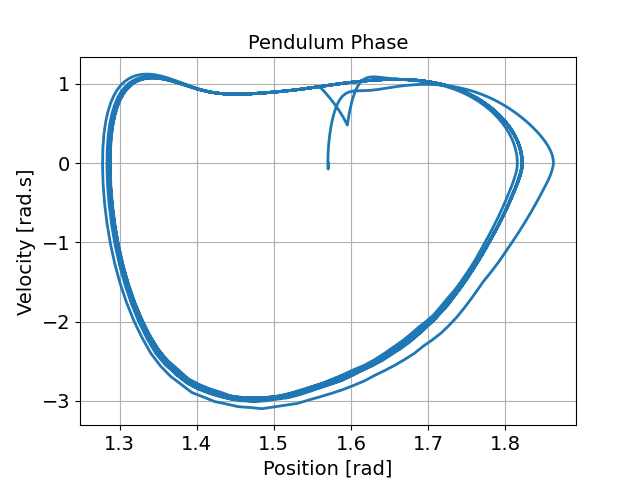
\includegraphics[width=0.99\textwidth]{figures/2b_sine_phased.png} }
    \caption{Phase diagram of the pendulum with the 1[Hz] phased square-shaped stimulation signal.}
    \label{fig:2b_sine_signal}
  \end{subfigure}
  \begin{subfigure}[b]{0.48\textwidth}
    { \centering
      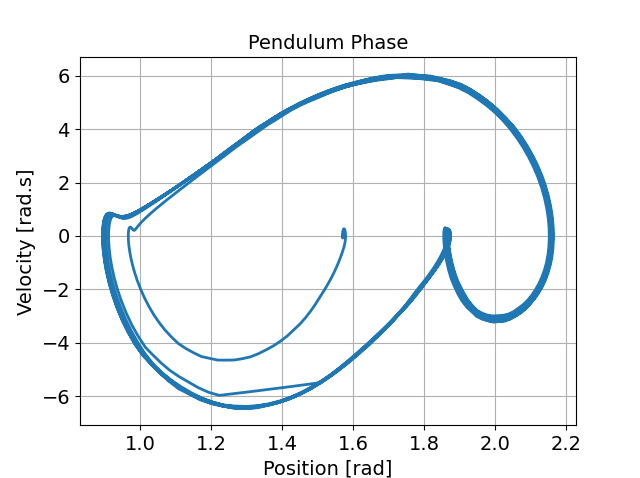
\includegraphics[width=0.99\textwidth]{figures/2b_sine_counterphased.png} }
    \caption{Phase diagram of the pendulum with the 1[Hz] counterphased sine-shaped stimulation signal.}
    \label{fig:2b_sine_phase}
  \end{subfigure}
  
  \begin{subfigure}[b]{0.48\textwidth}
    { \centering
      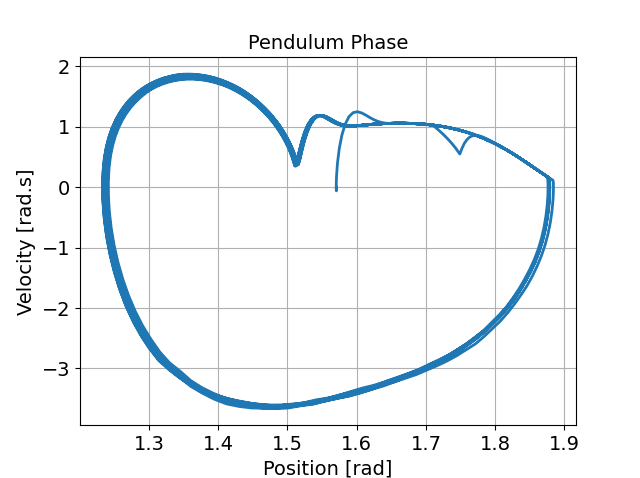
\includegraphics[width=0.99\textwidth]{figures/2b_square_phased.png} }
    \caption{Phase diagram of the pendulum with the 1[Hz] phased square-shaped stimulation signal.}
    \label{fig:2b_square_signal}
  \end{subfigure}
  \begin{subfigure}[b]{0.48\textwidth}
    { \centering
      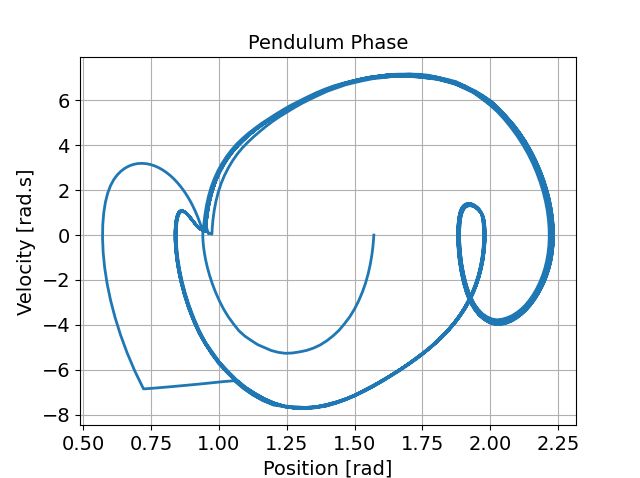
\includegraphics[width=0.99\textwidth]{figures/2b_square_counterphased.png} }
    \caption{Phase diagram of the pendulum with the 1[Hz] counterphased square-shaped stimulation signal.}
    \label{fig:2b_square_signal}
  \end{subfigure}
  
  \begin{subfigure}[b]{0.48\textwidth}
    { \centering
      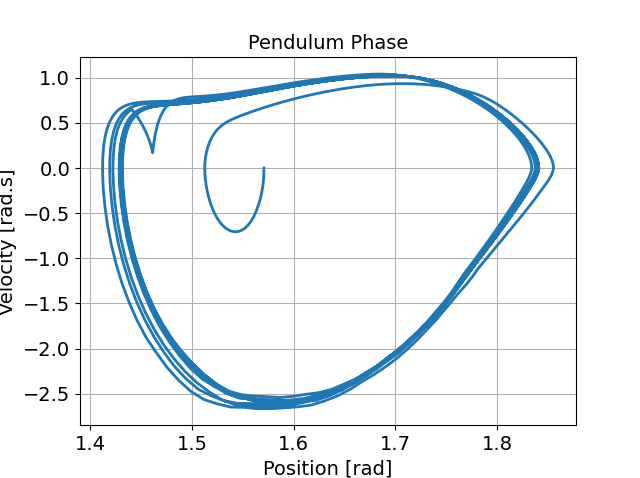
\includegraphics[width=0.99\textwidth]{figures/2b_sawtooth_phased.png} }
    \caption{Phase diagram of the pendulum with the 1[Hz] phased square-shaped stimulation signal.}
    \label{fig:2b_square_signal}
  \end{subfigure}
  \begin{subfigure}[b]{0.48\textwidth}
    { \centering
      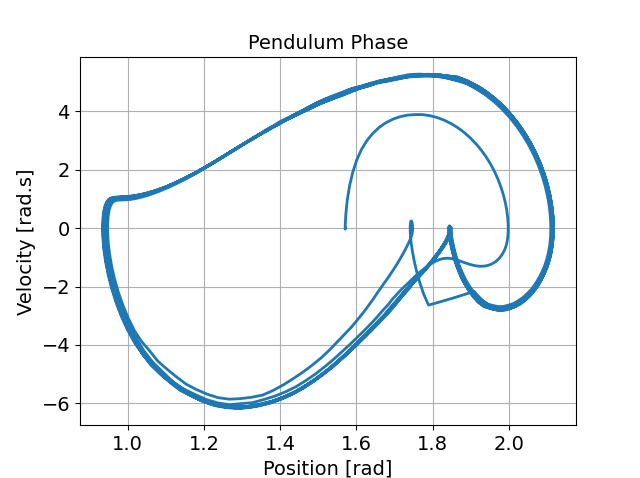
\includegraphics[width=0.99\textwidth]{figures/2b_sawtooth_counterphased.png} }
    \caption{Phase diagram of the pendulum with the 1[Hz] counterphased sawtooth-shaped stimulation signal.}
    \label{fig:2b_square_signal}
  \end{subfigure}
  \caption{Measurements of experiment 2b.}
  \label{fig:2b}
\end{figure}

%===========================================================
%END USER CODE
%===========================================================


\subsection*{2c. Explore the relationship between stimulation
  frequency with the resulting pendulum's behavior.  Report your
  inferences for a low and high frequency condition.  }
\label{sec:2c}

%===========================================================
%BEGIN USER CODE
%===========================================================

When we increase the frequency to 10[Hz], the limit circle tends to be much smaller and less clearly defined (less stable). We can suppose that the muscle is reached a state of "crispation" and has the time constant (inertia) of the system is too high to be able to follow precisely the stimulation variation (see Figure \ref{fig:2c_signals}). We also observe that the system takes more cycles to reach it.

\begin{figure}[H]
  \centering
  \begin{subfigure}[b]{0.48\textwidth}
    { \centering
      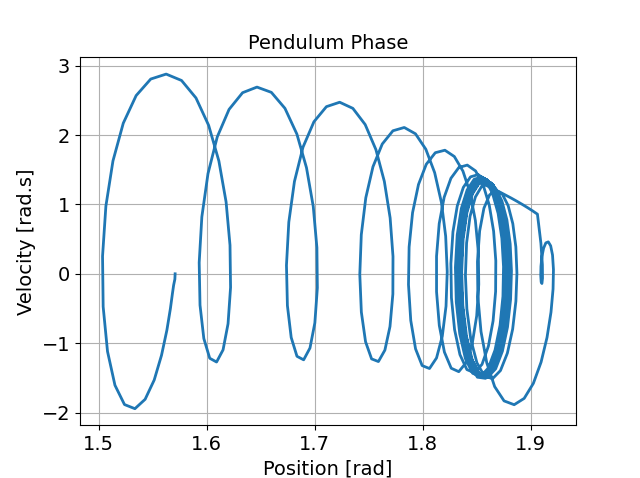
\includegraphics[width=0.99\textwidth]{figures/2b_sine_10HZ_counterphased.png} }
    \caption{Position-velocity behaviour with the Sine-shaped stimulation signal.}
    \label{fig:2c_sine_signal}
  \end{subfigure}
  \begin{subfigure}[b]{0.48\textwidth}
    { \centering
      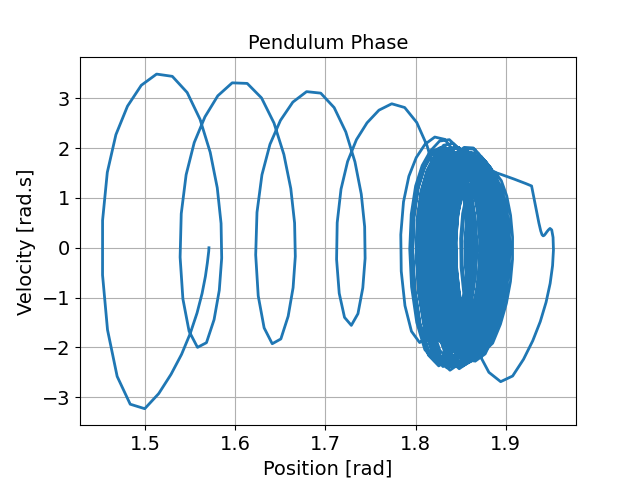
\includegraphics[width=0.99\textwidth]{figures/2b_square_10HZ_counterphased.png} }
    \caption{Position-velocity behaviour with the square-shaped stimulation signal.}
    \label{fig:2c_sine_phase}
  \end{subfigure}
  
  \begin{subfigure}[b]{0.48\textwidth}
    { \centering
      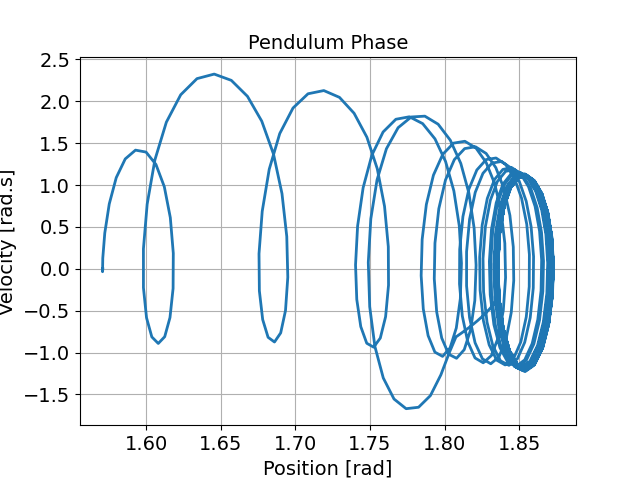
\includegraphics[width=0.99\textwidth]{figures/2b_sawtooth_10HZ_counterphased.png} }
    \caption{Position-velocity behaviour with the sawtooth-shaped stimulation signal.}
    \label{fig:2c_square_signal}
  \end{subfigure}

  \caption{Position-velocity behaviour of the system for each 10[Hz] signal. NOTE: for those three simulations, the flexor and extensor stimulation signals are counterphased.}
  \label{fig:2c_signals}
\end{figure}

%===========================================================
%END USER CODE
%===========================================================

\newpage
\section*{Exercise 3 : Neural network driven pendulum model with
  muscles}
\label{sec:neur-netw-driv}


\subsection*{3a. Find a set of weights and time constants for the
  neural network that produces oscillations to drive the pendulum into
  a limit cycle behavior. Plot the output of the network and the phase
  plot of the pendulum}
\label{sec:4a}

%===========================================================
%BEGIN USER CODE
%===========================================================

The selected parameters were taken from Lecture 4 on Neural Networks, slide 85:
\begin{center}
$
Weights =
\begin{pmatrix}
0 & -5 & -5 & 0\\
-5 & 0 & 0 & -5\\
5 & -5 & 0 & 0\\
-5 & 5 & 0 & 0
\end{pmatrix}
$
\end{center}

\begin{figure}[H]
 \centering
  \begin{subfigure}[b]{0.45\textwidth}
    { \centering
      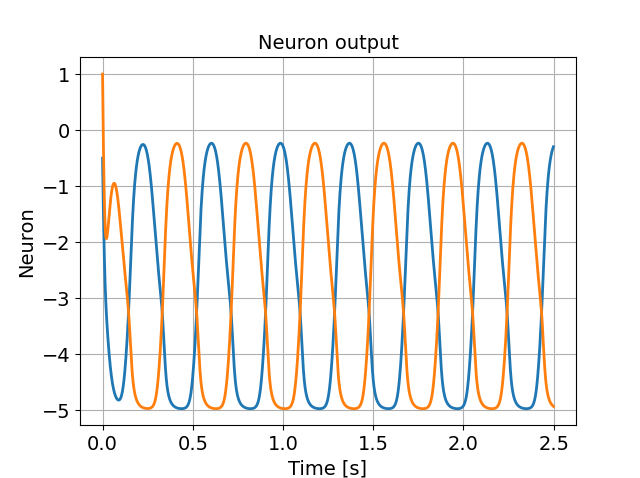
\includegraphics[width=0.99\textwidth]{figures/3a_neuron_output.png} }
    \caption{Neuron output of the network without any external drive}
    \label{fig:3a_neuron_output}
  \end{subfigure}
  \begin{subfigure}[b]{0.45\textwidth}
    { \centering
      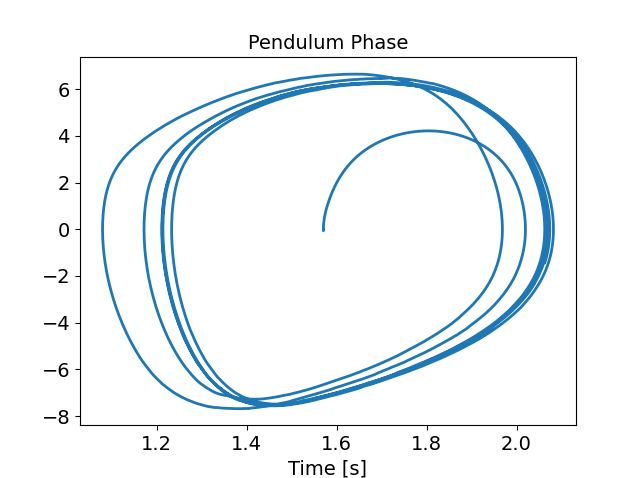
\includegraphics[width=0.99\textwidth]{figures/3a_pendulum_Phase.png} }
    \caption{Pendulum phase with our given parameters and no external drive.}
    \label{fig:3b_pendulum_phase}
  \end{subfigure}
  \caption{Measurements on the neural network with our weight matrix}
  \label{fig:3a}
\end{figure}

%===========================================================
%END USER CODE
%===========================================================



\subsection*{3b. As seen in the course, apply an external drive to the
  individual neurons and explain how the system is affected. Show
  plots for low [0] and high [1] external drives. To add external
  drive to the network you can use the method \\
  \fileref{system\_simulation.py::add\_external\_inputs\_to\_network}
}
\label{sec:4c}


%===========================================================
%BEGIN USER CODE
%===========================================================
\begin{figure}[H]
 \centering
  \begin{subfigure}[b]{0.45\textwidth}
    { \centering
      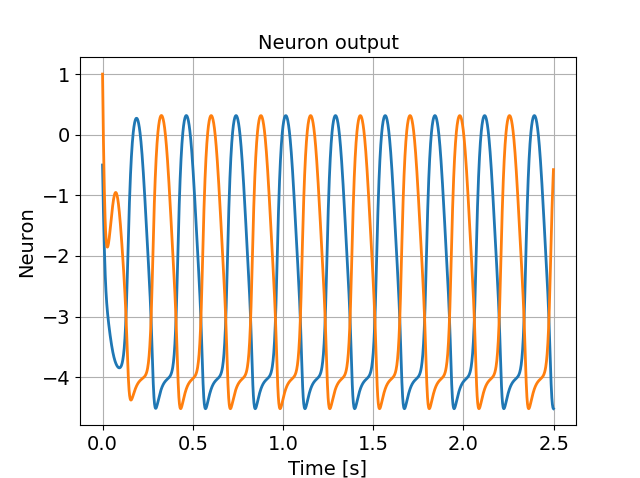
\includegraphics[width=0.99\textwidth]{figures/3b_1_neuron_output.png} }
    \caption{Neuron output of the network with an external drive gain of 1.}
    \label{fig:3b_1_neuron_output}
  \end{subfigure}
  \begin{subfigure}[b]{0.45\textwidth}
    { \centering
      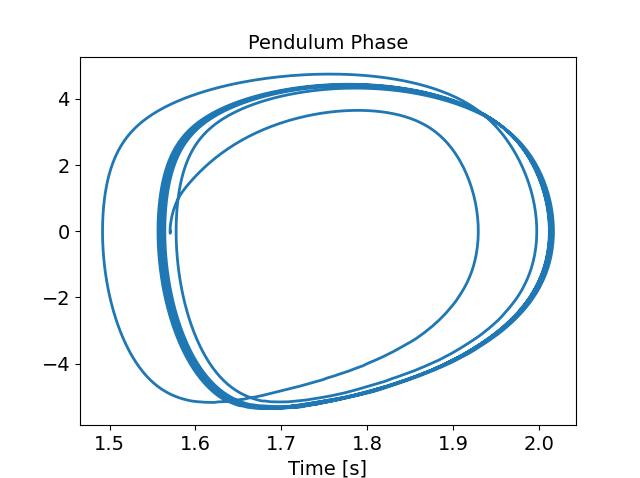
\includegraphics[width=0.99\textwidth]{figures/3b_1_pendulum_phase.png} }
    \caption{Pendulum phase with an external drive gain of 1.}
    \label{fig:3b_pendulum_phase}
  \end{subfigure}
  \begin{subfigure}[b]{0.45\textwidth}
    { \centering
      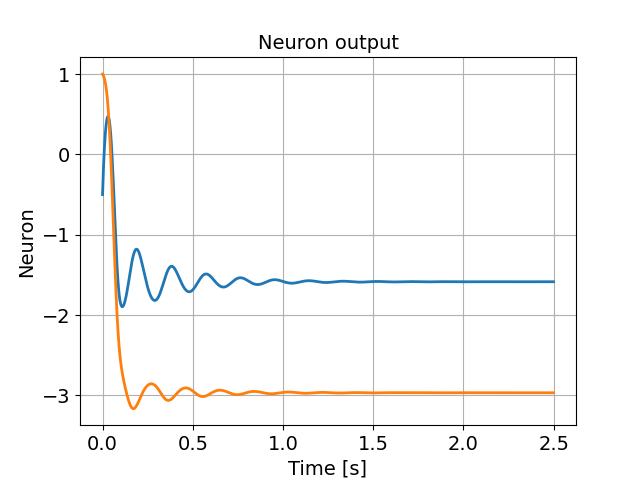
\includegraphics[width=0.99\textwidth]{figures/3b_6_neuron_output.png} }
    \caption{Neuron output of the network with an external drive gain of 6.}
    \label{fig:3b_1_neuron_output}
  \end{subfigure}
  \begin{subfigure}[b]{0.45\textwidth}
    { \centering
      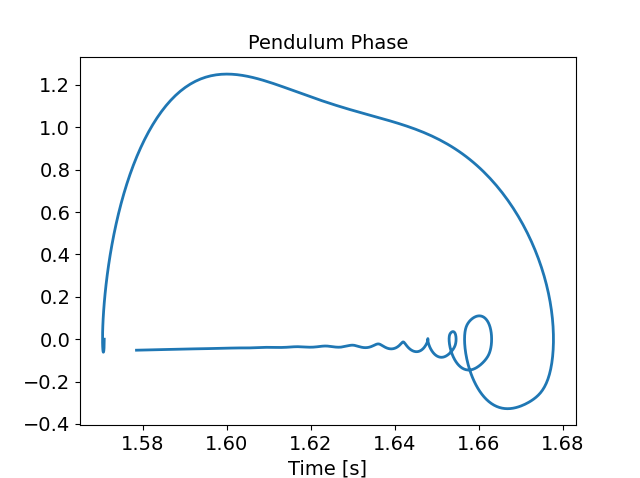
\includegraphics[width=0.99\textwidth]{figures/3b_6_pendulum_phase.png} }
    \caption{Pendulum phase with an external drive gain of 6.}
    \label{fig:3b_pendulum_phase}
  \end{subfigure}
  \caption{Measurements on the neural network with two different external drives.}
  \label{fig:3a}
\end{figure}

%===========================================================
%END USER CODE
%===========================================================


\subsection*{3c. [Open Question] What are the limitations of the half
  center model in producing alternating patterns to control the
  pendulum? What would be the effect of sensory feedback on this
  model? (No plots required)}
\label{sec:4d}

As we've observed in the experiment, a too high external drive can stop the generation of alternating patterns. Therefore, a sensory feedback high and long enough could "short-circuit" the neural system and stop the actuation (e.g. a high load on the motors) and render the robot motionless. It is also sensible to the starting position of the arm, and also the actuation symmetry is forced (we cannot stimulate each muscle independently).

\end{document}
